% Universidade Aberta
% Template TeX para relatório de trabalhos
% 2024
%
%
% Dados para a capa
\newcommand{\Titulo}{Diagramas de Componentes Git Activity Provider\\Antipadrões}
\newcommand{\Ano}{2025}
\newcommand{\Autor}{Hugo Gonçalves}
%
%
\documentclass[12pt,a4paper,final]{article}
\usepackage[stretch=10]{microtype}
\usepackage{csquotes}
\usepackage[portuguese]{babel}
\usepackage{polyglossia}
\setdefaultlanguage{portuguese}
\usepackage{graphicx}
\graphicspath{ {./images/} }
\usepackage[a4paper,top=3cm,bottom=3cm,left=3.5cm,right=2cm]{geometry}
\usepackage{booktabs}
\usepackage{newtxtext}
\usepackage{newtxmath}
\usepackage[pdfauthor=\Autor,
    pdftitle=\Titulo,
    colorlinks=true,
    linkcolor=black,
    citecolor=black,
    bookmarksopen=true]{hyperref}
\hypersetup{colorlinks, citecolor=black, urlcolor=black}
\usepackage{bookmark}
\usepackage{float}
\usepackage{tikz, tikz-uml}
\usepackage[style=apa, backend=biber, sortcites, url=true]{biblatex}
\addbibresource{ref.bib}
\renewcommand{\baselinestretch}{1.5}
\begin{document}
    \title{\Titulo}
    \author{\Autor}
    \date{\Ano}
    \pagenumbering{gobble}
    \begin{titlepage}
        \begin{center}
            \vspace*{4cm}

            \textbf{\large UNIVERSIDADE ABERTA}

            \textbf{\large UNIVERSIDADE DE TRÁS-OS-MONTES E ALTO DOURO}

            \vspace{1cm}

            \begin{minipage}{0.4\textwidth}
                \centering
                
\includegraphics[width=0.8\textwidth]{uab}
            \end{minipage}
            \begin{minipage}{0.4\textwidth}
                \centering
                
\includegraphics[width=0.8\textwidth]{utad}
            \end{minipage}

            \vspace{1.5cm}

            \textbf{\large \Titulo}

            \vspace{1.5cm}

            \textbf{\large \Autor}

            \vspace{2cm}

            \textbf{\large Mestrado em Engenharia Informática e Tecnologia Web}
            \vfill
            \textbf{\Ano}
        \end{center}
    \end{titlepage}
    \renewcommand{\contentsname}{Índice}
    \cleardoublepage
    \pagenumbering{roman}
    \listoffigures
    \newpage
    \cleardoublepage
    \pagenumbering{arabic}

    \noindent Identificou-se no AP \textit{Git Activity Provider} o antipadrão \textit{poltergeist} no serviço de configuração, pertencente ao componente de configuração.
    Na implementação atual deste componente, existem apenas duas funções: 1) fornecer os parâmetros de configuração e 2) fornecer a interface de configuração, correspondentes aos pedidos \textit{Configuration parameters} e \textit{Configuration Interface} da especificação da arquitetura Inven!RA segundo \cite{su15010857}.
    Uma vez que ambas as funções se limitavam a carregar do sistema de ficheiros o conteúdo a fornecer, é desnecessário existir um serviço dedicado bem como a \textit{Factory} para criar este serviço.
    Assim, a lógica de carregamento inicial foi movida para o \textit{Controller} e o serviço removido como se pode observar no \textit{commit} disponível em \href{https://github.com/2100562/GitActivityProvider/commit/5e78cf48587040aa2c1760b5d20ad858bd60c52e}{github.com/2100562/GitActivityProvider/commit/5e78..}.

    O diagrama de componentes geral do AP não foi alterado, no entanto, o diagram interno do componente de configuração foi simplificado.

    \begin{figure}[H]
        \centering
        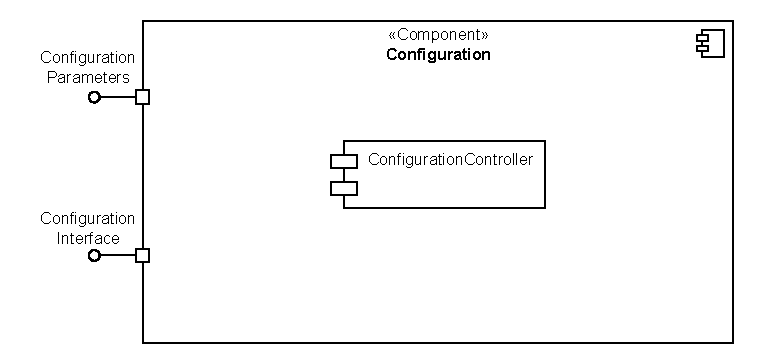
\includegraphics[width=\textwidth]{diagrama_componentes_v2-Configuration.drawio}
        \caption{Diagrama de Componentes - Componente de Configuração}
        \label{fig:dccc}
    \end{figure}

    \begin{figure}[H]
        \centering
        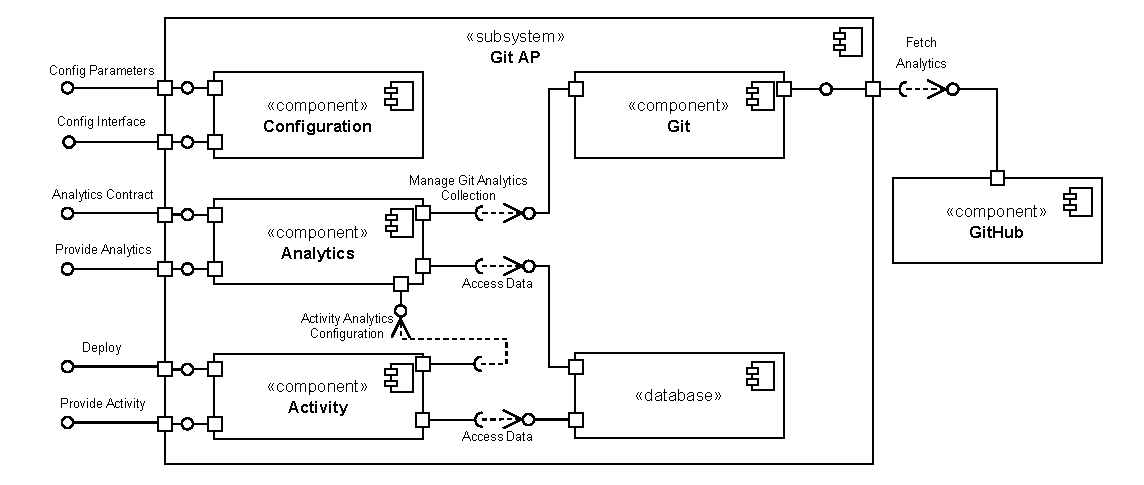
\includegraphics[width=\textwidth]{diagrama_componentes_v2-AP.drawio}
        \caption{Diagrama de Componentes - Git Activity Provider}
        \label{fig:dcgap}
    \end{figure}

    \noindent As alterações descritas acima, permitiram, também simplificar o diagrama de sequência.

    \begin{figure}[H]
        \centering
        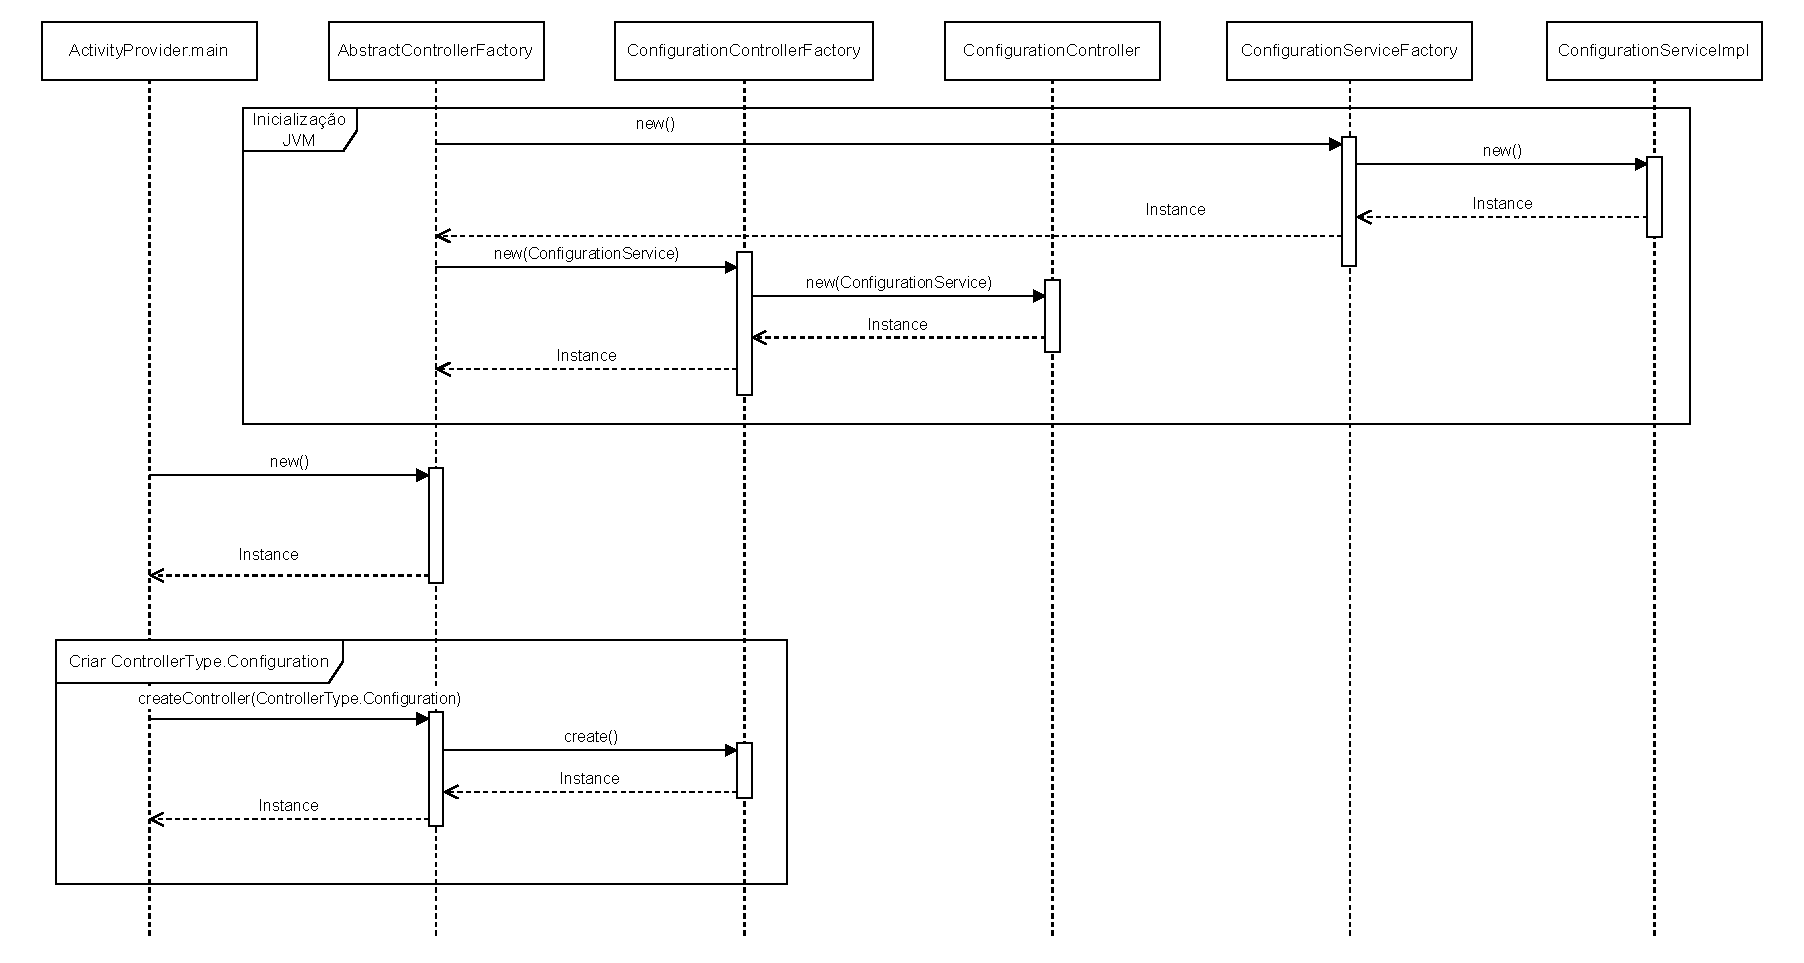
\includegraphics[width=\textwidth]{diagramas_padroes_criacao-old.drawio}
        \caption{Diagrama de Sequência - Configuration Controller, antigo}
        \label{fig:dscca}
    \end{figure}

    \begin{figure}[H]
        \centering
        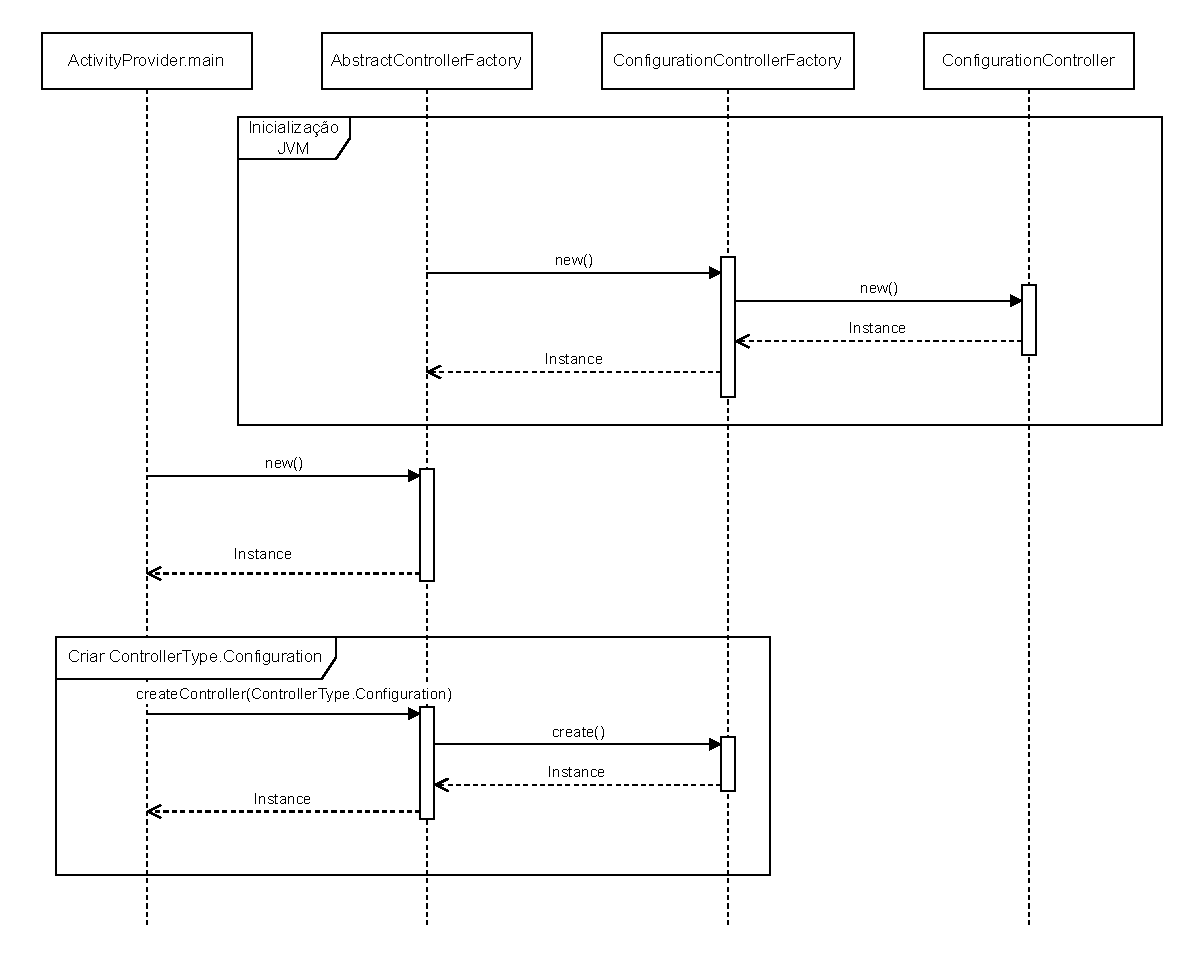
\includegraphics[width=\textwidth]{diagramas_padroes_criacao-new.drawio}
        \caption{Diagrama de Sequência - Configuration Controller, novo}
        \label{fig:dsccn}
    \end{figure}

    \newpage
    \printbibliography
\end{document}
